\chapter[The runtime database]{The runtime database} \label{ch:rtdb}

\section{Schematic overview}

\begin{figure}[\htb]
  \centering
  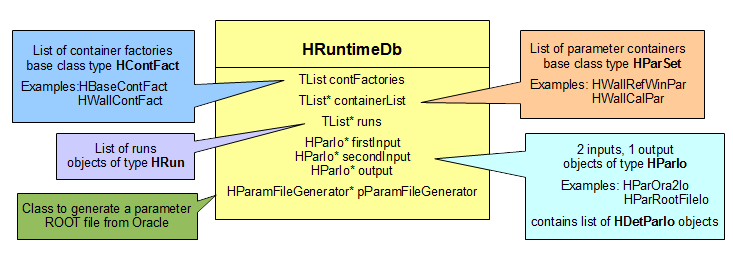
\includegraphics[scale=0.75]{hydra2_rtdb_classdiagram.png}
  \caption[HRuntimeDb class diagram]{HRuntimeDb class diagram} \label{fig:rtdbHRuntimeDbClassDiagram}
\end{figure}

\paragraph{Features:} ~\\
The parameters are stored in parameter containers (see \ref{sec:rtdbParamContainers})\\
The runtime database allows to create all parameter containers via the container factories 
(see~\ref{sec:rtdbContainerFactories}).\\
Once a parameter container is created, it is added in the list of parameter containers and accessible in Hydra2 by all 
tasks, which need these parameters.\\
The runtime database allows to specify one or two input sources and takes care, that the parameters are initialized at 
the beginning of each run with the appropriate version (see~\ref{sec:rtdbParameterIo}). \\
The user may specify an output and the runtime database takes care, that the parameters are automatically written to   
this output before the parameter container is initialized again or before it is deleted.\\
For each run it stores for each parameter container the input and output versions. This run catalog is, together 
with the detector setups, written to the ROOT file output to be used as a local database for initialization 
(see~\ref{sec:rtdbHParRootFileIo}).\\
For Oracle as input it allows to create a parameter ROOT file for all runs of a specified beam time and time range 
(see \ref{sec:rtdbHParamFileGenerator}).

\subsection[The building blocks for parameter initialization and output]
           {The building blocks for parameter initialization and output}

\paragraph{Loading the HYDRA libraries} ~\\
When the shared libraries are loaded in ROOT, the container factories are created and added to the list of container 
factories in the runtime database, which is implemented as a singleton.

\paragraph{Create Hades} ~\\
The \verb+Hades+ constructor instantiates the runtime database (class \verb+HRuntimeDb+) and creates an object 
of class \verb+HSpectrometer+.\\
\begin{lstlisting}
  Hades* myHades = new Hades;
  HSpectrometer* spec = gHades->getSetup();
  HRuntimeDb* rtdb = gHades->getRuntimeDb();
\end{lstlisting}

\begin{figure}[\htb]
  \centering
  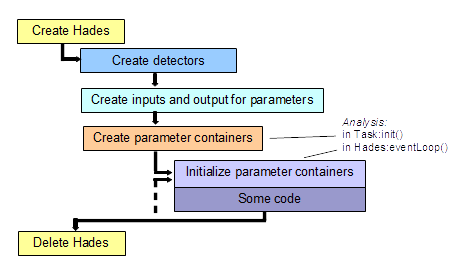
\includegraphics[scale=0.75]{hydra2_rtdb_flowchart.png}
  \caption[Flow chart of initialization]{Flow chart of initialization} \label{fig:rtdbFlowChart}
\end{figure}

\paragraph{Create detectors} ~\\
In the analysis one must create all detectors with their appropriate setup.\\
In an initialization macro it is also mandatory for all tree-style parameter containers because they use detector 
specific I/O classes. Condition-style parameter containers use a base class I/O interface, a detector is not needed.\\

Each detector has its own class (\verb+HMdcDetector+, \verb+HWallDetector+, \ldots). They are all derived from the base 
class \verb+HDetector+. Each detector consists of one or more modules placed in the different sectors or directly in the cave.\\

The code snippets below creates the Forward Wall detector (with sector = -1, because it sits in the cave) and the MDC detector 
with 6 sectors, but one module missing (0 = module is absent, 1 = module in setup), and adds them to the list of detectors 
in the \verb+HSpectrometer+ object.
\begin{lstlisting}
  HWallDetector* wall=new HWallDetector;
  Int_t wallMods[]={1};
  wall->setModules(-1,wallMods);
  spec->addDetector(wall);

  HMdcDetector* mdc=new HMdcDetector;
  Int_t mdcMods[6][4]={ {1,1,1,1},
                        {1,1,1,1},
                        {1,1,0,1},
                        {1,1,1,1},
                        {1,1,1,1},
                        {1,1,1,1} };
  for(Int_t i=0;i<6;i++) { mdc->setModules(i,mdcMods[i]); }
  spec->addDetector(mdc);
\end{lstlisting}

\paragraph{Create input and output for parameters} ~\\
Here one creates the data sources for the parameters and sets them as first or second input in the runtime database.\\
Additionally one may specify an output.\\
Possible I/O types are Oracle, ROOT files, ASCII files.\\

Typically one uses two inputs
\begin{itemize}
  \setlength{\itemsep}{0pt}    
  \item if one wants to merge the data from two input sources into one ROOT file
  \item if one has some parameters in a file (set this as first input) not stored in Oracle, but all others should be
        read from Oracle (set as second input)
\end{itemize}

There is a \textbf{simple rule}:\\
If a parameter container can be initialized from the first input, the second input is not used for this container.\\

For a more detailed description of the parameter I/O classes and features see \ref{sec:rtdbParameterIo}.\\
Here only a small example, which reads the data from Oracle and writes them to a ROOT file:

\begin{lstlisting}
  HParOra2Io* ora=new HParOra2Io;
  ora->open();
  rtdb->setFirstInput(ora);

  HParRootFileIo* output=new HParRootFileIo;
  output->open("params.root","RECREATE");
  rtdb->setOutput(output);
\end{lstlisting}

\paragraph{Create parameter containers} ~\\
Typically parameter containers are created by the parameter container factories in the runtime database.\\
If one wants to use a non-default context for a parameter container, one should set it before the parameter container 
is created (see~\ref{sec:rtdbContainerFactories}).
\begin{lstlisting}
  Bool_t HRuntimeDb::addParamContext(const char context)
\end{lstlisting}

One creates the containers with
\begin{lstlisting}
  HParSet* HRuntimeDb::getContainer(Text_t containerName);
\end{lstlisting}
The function checks if the container exists already and, if not, creates it. It returns a pointer to the parameter 
container, but with the base class type, and it must be casted to the concrete type to use the functions not available 
in the base class, for example:
\begin{lstlisting}
  HWallRefWinPar* pPar=(HWallRefWinPar*)(rtdb->getContainer("WallRefWinPar"));
\end{lstlisting}

One may also create the parameter container via the constructor, but then one must also add it to the runtime database 
to be later automatically initialized, stored in the output and finally deleted.

\begin{lstlisting}
  HWallRefWinPar* pPar=new HWallRefWinPar();
  rtdb->addContainer(pPar);
\end{lstlisting}

In the analysis the parameter containers are created typically in the init functions of the tasks (called in 
\verb+Hades:init()+).\\
A few of them are also initialized, for example parameter containers needed to create other parameter containers or to 
create the data structure for the unpackers. But these are exceptions.

\paragraph{Initialize parameter containers} ~\\
All parameter containers can be initialized with the function call
\begin{lstlisting}
  Bool_t HRuntimeDb::initContainers(Int_t runId, Int_t refId, const Text_t fileName);
  // runId     number in the event header uniquely defining the hld file or simulation run
  // refId     reference run id (default value: -1)
  //           if != -1, all containers are initialized with the versions valid for this run
  // fileName  name of current event file (default NULL)
\end{lstlisting}
This function is automatically called in the Hades event loop for the first event of each file.\\
In a macro it must be called explicitly (eventually several times with different run ids).\\
The function loops over all parameter containers and calls their init function (see \ref{sec:rtdbHParSet} for 
details).\\

In the analysis, the reference run id is set in the data source of the events and always necessary, if parameters are 
not available for the file to be analyzed. One example are simulation runs where the simulation reference run was 
\textbf{not} set in the configuration file (see \ref{sec:geomGeainiKeywords} for details).

\paragraph{Delete Hades} ~\\
Before one deletes the Hades object and with it the runtime database, one may want to see its content (in principle 
one can do this everywhere in the macro, even multiple times)
\begin{lstlisting}
  rtdb->saveOutput();
  rtdb->print();
\end{lstlisting}

The function \verb+HRuntimeDb::saveOutput()+ loops over all parameter containers and writes them to the output if 
not yet done. For a ROOT file as output, it also writes the detector setups and the version table, which contains 
for each run the two input and the output versions, into the output file. Only the output versions are stored in the file. 
These will be the input versions for the runs when the ROOT file is used as input.\\

The function \verb+HRuntimeDb::print()+lists the parameter containers, the version table and information about the 
input(s) and output. (see Example ~\ref{sec:rtdbSimpleMacro})\\
\textbf{Warning:} If one calls this function without calling \verb+rtdb->saveOutput()+ before, the version table might be 
misleading, because the input and output versions are stored in the version table when the write function is called and 
for the current run this might have not been done yet.


\subsection{A simple initialization macro} \label{sec:rtdbSimpleMacro}

This macro initializes the parameter container HMagnetPar, which contains the magnet current, from Oracle for three runs 
in beam time APR12 and writes it to a ROOT file.
\begin{lstlisting}
{
  // create the Hades object and get the pointer to the runtime database  
  Hades* myHades=new Hades;
  HRuntimeDb* rtdb=gHades->getRuntimeDb();

  // define the input
  HParOra2Io* input = new HParOra2Io;
  input->open();
  rtdb->setFirstInput(input);

  // define the output
  HParRootFileIo* output = new HParRootFileIo;
  output->open("test.root","RECREATE");
  rtdb->setOutput(output);

  // create the parameter container(s)
  HMagnetPar* pMagnetPar = (HMagnetPar*)(rtdb->getContainer("MagnetPar"));

  // initialize the parameter container
  rtdb->initContainers(133602648);  // magnet off
  rtdb->initContainers(133656363);  // magnet on
  rtdb->initContainers(133656526);  // magnet on  
  
  // print the parameters on the screen  
  pMagnetPar->printParams();

  // save the output (writes the data to the file)
  rtdb->saveOutput();

  // print content of the runtime database on the screen
  rtdb->print();

  // delete the Hades object
  delete myHades;
}
\end{lstlisting}

Result of \verb+rtdb->initContainers(133602648);+
\begin{lstlisting}
************************************************************

   info<HRuntimeDb>:  initialisation for run id 133602648
************************************************************

*************************************************************
     Oracle history date: 10-JUL-2015 22:13:30
*************************************************************
MagnetPar initialized from Oracle
\end{lstlisting}
When called the first time the history date, here the last parameter release for beam time APR12, is set.
Then the parameter container is initialized.\\

Result of \verb+rtdb->initContainers(133656363);+
\begin{lstlisting}
   info<HRuntimeDb>: MagnetPar written to ROOT file, version: 1
************************************************************

   info<HRuntimeDb>:  initialisation for run id 133656363
************************************************************

MagnetPar initialized from Oracle
\end{lstlisting}
First the parameter container is written to the output with version number 1, then it is initialized for the next run. 
The magnet current is different. This leads to a new version.\\ 

Result of \verb+rtdb->initContainers(133656526);+
\begin{lstlisting}
   info<HRuntimeDb>: MagnetPar written to ROOT file, version: 2
************************************************************

   info<HRuntimeDb>:  initialisation for run id 133656526
************************************************************
\end{lstlisting}
The parameter container is written to the output with version number 2, then it is initialized for the next run. Because 
the start time of this run is in the validity time range of the version read for the previous run, the input version 
is the same. The Oracle read function is not even called.\\

Result of \verb+pMagnetPar->printParams();+
\begin{lstlisting}
---------------------------------------------
-----  MagnetPar  -----
--  Context/Purpose:  MagnetCurrentSetValues
--  Description:      Read from Oracle
             Valid for Run Id 133656363
             Status at 10-JUL-2015 22:13:30
---------------------------------------------
current: Int_t   2500 
---------------------------------------------
\end{lstlisting}

The call of \verb+rtdb->saveOutput()+ does not print anything on the screen because the last version was already written 
into the file. The write function of the parameter container only stores also for this run the last output version in the version table.\\ 

Result of \verb+rtdb->print();+
\begin{lstlisting}
------------------------------------------------------------

   info<HRuntimeDb>: actual containers in runtime database
   info<HRuntimeDb>: MagnetPar          Magnet current
   info<HRuntimeDb>: runs, versions
--------------------------------------------------------------------------------

   info<HRuntimeDb>: run id
----------------------------------------

   info<HRuntimeDb>: container              1st-input 2nd-input    output
   info<133602648>: run: 133602648
   info<133602648>: MagnetPar              133602648         -1        1
   info<133656363>: run: 133656363
   info<133656363>: MagnetPar              133656363         -1        2
   info<133656526>: run: 133656526
   info<133656526>: MagnetPar              133656363         -1        2
--------------------------------------------------------------------------------

   info<HRuntimeDb>: input/output
----------------------------------------

   info<HRuntimeDb>: first Input:
Oracle-Database: db-hades    Username: hades_ana
History date: 10-JUL-2015 22:13:30
Hydra2 Oracle interface
detector I/Os:  HCondParIo HSpecParIo
--------------------------------------------------------------------------------

   info<HRuntimeDb>: second Input: none
--------------------------------------------------------------------------------

   info<HRuntimeDb>: Output:
HParRootFile**          test.root
 HParRootFile*          test.root
  KEY: HMagnetPar       MagnetPar;2     Magnet current
  KEY: HMagnetPar       MagnetPar;1     Magnet current
  KEY: HRun     133602648;1
  KEY: HRun     133656363;1
  KEY: HRun     133656526;1
detector I/Os:  HCondParIo HSpecParIo
\end{lstlisting}

Result of \verb+delete myHades;+
\begin{lstlisting}
connection to Oracle closed
\end{lstlisting}

This ROOT file can be used as input to initialize the parameter containers for the three run ids in the ROOT file.\\
Other runs with the same field settings can only be initialized by using one of these run ids as 
\textbf{reference run id}, for example
\begin{lstlisting}
    Int_t refRunId=133656363;
    rtdb->initContainers(133656688,refRunId); // also magnet on 
\end{lstlisting}
The container will be initialized for run 133656688 with the same data as for 133656363 (version 2).


\subsection{Initialization in an analysis macro}

In the following only the parts relevant for initialization are described (\textbf{without using the DST library}).

One creates in the macro the detectors, the parameter input(s) and eventually a parameter output.\\
Then one defines the data source(s) and adds one or more files, eventually with a reference run. The data source opens 
the first file and reads the run id in the header. If a reference run is defined by filename, it opens also this file 
and reads its run id.\\
For HLD files one also adds the unpackers in the HLD source.\\
Then one defines the tasks respectively task sets.\\

The parameter containers are created when \verb+Hades::init()+ is called:
\begin{enumerate}
  \setlength{\itemsep}{0pt}    
  \item Initializes all containers already created.
  \item Calls the init function of all detectors\\
        For the MDC the parameter containers \verb+HMdcRawStruct+ and \verb+MdcGeomStruct+ are created and initialized 
        (needed to build other parameter containers and the data structures).
  \item Calls the init functions of the data sources\\
        The init function of a HLD source calls the init function of all unpackers, where the lookup tables are created.
  \item Calls the init function of all tasks. Here all other parameter containers are created.
\end{enumerate}

At this point all parameter containers are in the runtime database, but besides a few exceptions, 
\textbf{not yet initialized}.\\
This is done in the \textbf{Hades event loop}:
\begin{enumerate}
  \setlength{\itemsep}{0pt}    
  \item Before analyzing the first event of a file all containers are initialized.
  \item Then the connection to Oracle is closed.
  \item The re-init function of all tasks is called.\\
        Some tasks calculate private data from the parameter containers and use them in the execute function.\\
        If several files are analyzed in a chain (or for a ROOT file as input generated from several input files) step 
        1 - 3 is repeated. The connection to Oracle is automatically re-opened and closed again after initialization.
\end{enumerate}

If one wants to change parameters in a container on-the-fly in the macro without creating a parameter file before 
one can do this directly before the Hades event loop:
\begin{itemize}
  \setlength{\itemsep}{0pt}    
  \item One gets the pointer to the parameter container using the function\\
        \verb+HParSet* HRuntimeDB::findContainer(Text_t* containerName)+.\\
        It returns the pointer to an existing container (the constructor is not called).
  \item One initializes the parameter container (by calling its \verb+init()+ function)
  \item Now one changes the parameter(s).
  \item The parameter container must be set static to avoid a re-initialization\\ 
        (by calling its function \verb+setStatic(Boot_t flag=kTRUE)+.
\end{itemize}


\section[Parameter containers]{Parameter containers} \label{sec:rtdbParamContainers}

%The parameters are stored in parameter containers, which are managed by the runtime database and %accessible via their names. 
%They are all derived from the base class \textbf{HParSet}.
%

\subsection[Base class HParSet]{HParSet, the base class for all parameter containers} \label{sec:rtdbHParSet}

This class defines the common data elements, some basic functionality and the virtual functions each container class must 
implement for initialization and output.

\paragraph{Data Members of HParSet:}
\begin{itemize}
 \item \verb+TString fName, TString fTitle+\\
   HParSet is derived from the ROOT class \textbf{TNamed} and inherits its data members. The name uniquely identifies the 
   container in the runtime database.
 \item \verb+TString paramContext+\\
   This is the name of the parameter context. A parameter context allows to support different flavors of the parameters, 
   which are valid for the same run start\footnote{Beam and simulation runs may have the same run start, but the parameters 
   might be different. To distinguish between them in Oracle, the identifier of the context id is different for the 
   two run types, but the name is the same.}. The context defined in the constructor is the default context. Others might be set 
   either via the container factory or explicitly in the macro.
 \item \verb+Bool_t status+\\
   By default this flag is kFALSE and the parameters are initialized for each run. Once set kTRUE, the container is skipped 
   in the automatic initialization in the runtime database.\\
   Member functions:\\
   \verb+    void   setStatic(Bool_t flag=kTRUE);+\\
   \verb+    Bool_t isStatic();+
 \item \verb+Bool_t changed+\\
   By default this flag is kFALSE and set kTRUE after each initialization, which signals, that the container must be written 
   to the output before the data are overwritten by the next initialization or before the container is deleted. The write 
   function then again resets the flag.\\
   Member functions:\\
   \verb+    void   setChanged(Bool_t flag=kTRUE);+\\
   \verb+    Bool_t hasChanged()();+
 \item \verb+Int_t versions[3]+\\
   It stores in versions[1] the version number from the first input, in versions[2] the one from the second input.\\
   By default all versions are -1 (not initialized). If both version numbers are -1 after initialization, the parameter 
   container is not written to the output.\\
   If one fills the parameter container in the macro and not via the runtime database, versions[1] must be set to 1.\\ 
   Member functions:\\ 
   \verb+    void  setInputVersion(Int_t v=-1,Int_t i=0);+\\
   \verb+    Int_t getInputVersion(Int_t i);+\\
   The function \verb+void resetInputVersions()+ sets all input versions to -1 and the status flag to kFALSE, but only for 
   a non-static parameter container (status flag kFALSE). 
 \item \verb+Text_t detName[20]+\\
   This is the name of the detector the container belongs to and set in the constructor of the derived class.\\
   It is mandatory for all parameter containers which might initialize only a subset of the modules or want to check if all 
   modules in the setup are initialized. Geometry containers need it to retrieve the detector name and setup from Oracle.
 \item \verb+TString author, TString description+\\
   These are the author and the description of the parameters in Oracle. They must be filled before the data can be written into 
   Oracle.
\end{itemize}

\paragraph{Functions implemented in the base class:}
\begin{itemize}
  \item \verb+virtual Bool_t init(HParIo*);+\\
    If the detector name is defined, it first creates an array corresponding to the setup array of this detector.\\
    Then it checks, if the parameter container was initialized the last time from two inputs and in this case it resets 
    the input versions.\\
    After this it tries to initialize the parameter container from the first input (if defined) in the runtime database by 
    calling the init function in the derived class (described below). If this fails, because the input cannot provide the data 
    or not all of them, it calls also the init function for the second input (if defined).\\
    If the parameter container is then still not fully initialized it returns kFALSE, otherwise kTRUE.
  \item \verb+virtual Int_t write();+\\
     This function gets the output pointer from the runtime database and, if defined, with this calls the function
     in the derived class (described below).
  \item \verb+void print();+\\
  It prints information about the container (context, author, description, versions, status, changed ...).
\end{itemize}

\paragraph{Functions implemented in the derived class:}
\begin{itemize}
  \item \verb+virtual Bool_t init(HParIo*,Int_t*);+\\
    This function initializes the container from an input using the detector specific
    interface class of type HDetParIo (see section \ref{sec:rtdbParameterIo} for details).
  \item \verb+virtual Int_t write(HParIo*);+\\
    It writes the container to an output using the detector specific interface class of type HDetParIo.\\
    If one wants to write a parameter container into Oracle, one must use this write function with the pointer to the Oracle 
    output as parameter. One cannot use the base class write function without an argument.
  \item \verb+void clear();+\\
    This function resets the parameters to the default values and sets the input/output versions to -1.
\end{itemize}

\subsection[Tree-style parameter containers]{Tree-style parameter containers} \label{sec:rtdbTreeStyleParamCont}
These parameter containers are directly derived from HParSet. Some of them have a tree-like class structure.\\ 
Since 2002 we use a standardized table layout in Oracle for a certain group of parameter containers:
\begin{itemize}
 \item They have a tree-like structure: sector, modules, ..., cells.
 \item Typically they hold a large amount of data.
 \item They might be closely related to hardware modules (the data stick to the hardware module, not to the position of this module).
 \item They need a version management.
 \item The data elements will probably not change anymore in future code releases.
 \item The data consistency is checked in Oracle via constraints.
\end{itemize}
Typical examples are the low-level parameter containers as unpacker lookup tables, thresholds, calibration parameters, \ldots.\\

Although the parameters themselves are individual (they may even be stored in several tables), they use a standard layout for 
the version management.
\begin{itemize}
  \item \textbf{Advantage:}
    \begin{itemize}
      \item This allows to write parts of the analysis interface code with cut-and-paste or to reuse code (even without 
            using dynamic SQL for performance reasons).
      \item It is possible to use a \textbf{generic WebDB GUI} for validation and queries.
      \item In the ASCII interfaces one can at least partially use template functions for read/write.
    \end{itemize}
  \item \textbf{Disadvantage:}
    \begin{itemize}
      \item It needs more coding.
      \item The Oracle tables, views, interfaces need to be implemented and later eventually changed by an expert.
    \end{itemize}
\end{itemize}


\subsection[Condition-style parameter containers]{Condition-style parameter containers} \label{sec:rtdbCondStyleParamCont}
If the list of data members of a tree-like parameter container changes, the ``expert`` must change the Oracle part.
This type is therefore not appropriate for parameter containers as for example conditions (this lead to the name) used 
in high level analysis, where the code is not stable and may change with every major code release.\\

To overcome this problem a new type of parameter container has been developed. The data are stored in a generic way 
in Oracle and the interfaces for Oracle, ROOT  and ASCII files are almost completely implemented in base classes.
\begin{itemize}
  \item \textbf{Advantage:}
    \begin{itemize}
      \item Minimizes code development
      \item No need for any new development in Oracle (no expert needed)
      \item Properly implemented, it is almost code independent. People can use old \textbf{and} new code to read the 
            data from Oracle.
      \item Allows to store also large arrays or even ROOT objects in binary format and to read these data very fast.
    \end{itemize}
  \item \textbf{Disadvantage:}
    \begin{itemize}
      \item All parameters are independent. One cannot put any constraints on the data in Oracle. Consistency checks
            need to be implemented in the code of the parameter container.
    \end{itemize}
\end{itemize}

The parameter container must inherit from \textbf{HParCond}, derived by itself from HParSet.\\
Three functions must be implemented:
\begin{enumerate}
 \item \verb+void clear(void);+\\
       This function is called automatically before an initialization (new version of parameters). 
 \item \verb+void putParams(HParamList*);+\\
       It fills all persistent data members into the list for writing (for Oracle and ASCII files).                                                   
 \item \verb+Bool_t getParams(HParamList*)+\\
       It fills all persistent data members from the list after reading. It returns false, when the data of a data member 
       is not in the list.
\end{enumerate}

The Oracle and ASCII read interface fills \textbf{all} valid parameters for the parameter container into a list in class 
\textbf{HParamList} (with list elements of type \textbf{HParamObj}) used for transfer. The \verb+getParams+ function takes from the list only the parameters in the 
actual used code version calling overloaded functions for the different parameter types.\\
See class documentation for details.\\

ALL data are stored in Oracle as binaries (small amount of data in RAW format, larger ones as Binary Large Objects 
(BLOBS). For ROOT objects (Hydra2 classes derived from TObject) also the streamer info is stored.

\paragraph{Design considerations:} ~\\
Try to avoid the use of ROOT objects in HParamList because they cannot be inspected by the ORACLE WebDB interface and they 
cannot be stored in an ASCII file. Histograms for example can be serialized into a TArrayD with the HHistConverter before putting 
them to the list. An example is the parameter container HParticleCandFillerPar.\\


\section[Parameter container factories]{Parameter container factories} \label{sec:rtdbContainerFactories}

Each library, which contains parameter container classes, must also contain a parameter container factory, derived
\textbf{HContFact}. It is created when the library is loaded into ROOT and added to the list of container factories 
in the runtime database.\\

Each factory contains the list of parameter container names and possible contexts in the corresponding library.\\
Examples: \verb+HBaseContFact+ contains all parameter containers in libBase, \verb+HRichContFact+ the ones in libRich.

\subsection*{Functionality}

\begin{itemize}
 \item They allow to create the parameter containers via the function call:\\
   \verb+    HParSet* getContainer(const char* containerName);+  
 \item For each parameter container they know the possible contexts and they take care for the name of the container when 
   it is created.\\
   Having different names, they can be read and written from/to the same ROOT file without the need to change the 
   version management.\\
   Naming convention:
   \begin{itemize}
     \item If no context was specified before, the parameter container is created with its default context and the 
       name is the standard name.
     \item For non-default contexts, the name of the parameter container is concatenated as\\
       "standard container name" + "\_" + "context name"
    \end{itemize}
 \item Different, but somehow related containers may share the same context.\\ 
   Setting this context only once guarantees that all these containers are initialized consistently.
   For example all geometry containers share the same context ''GeomProduction``.
\end{itemize}

\subsection*{Usage}

The user typically does not access the container factory directly in the macro, but calls functions in the runtime database:\\

\verb+Bool_t HRuntimeDb::addParamContext(const char* context)+\\
This function sets the context of all parameter containers, which accept this context. If a parameter container is 
created later by the factories it will be created with this context.\\

\verb+HParSet* HRuntimeDb::getContainer(Text_t* standardContainerName)+\\
The function loops over all container factories to find the factory responsible for the parameter container with the specified 
name. The factory then checks, if a special context is set, eventually concatenates the name and then checks, if a container 
with this name eventually exists already in the runtime database. If not, it creates the container and adds it in the runtime 
database.\\
The function returns the pointer to the container, which must be casted to the special container class type. It returns NULL, 
if the container was not created.


\section[Parameter input/output]{Parameter input/output} \label{sec:rtdbParameterIo}

\subsection[Class Design]{Class Design}

The class design for I/O was developed according to the following requirements:
\begin{itemize}
 \item Provide interfaces to Oracle, ROOT files and ASCII files
 \item To avoid dependencies, each detector has its own classes implementing the concrete read and write functions
 \item The actually used I/O is specified in the macro.
 \item The interface to Oracle is a shared library not included by the other libraries, except libDst.\\
   To compile this library one needs the Oracle client, which might not be installed.
\end{itemize}

\begin{figure}[\htb]
  \centering
  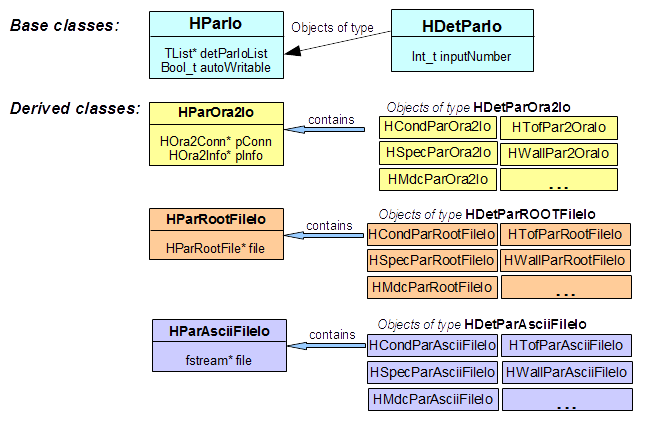
\includegraphics[scale=0.8]{hydra2_ioclasses}
  \caption[Hydra2 I/O classes]{Hydra2 I/O classes} \label{fig:paramInitHydra2IoClasses}
\end{figure}

The base class \textbf{HParIo} defines the virtual functions each type of I/O must implement, for example to close the I/O 
or to check, if the I/O is open.\\

The derived classes implement the open function (different arguments for the different types). This class is instantiated 
in the macro and then set as input or output in the runtime database.\\
It inherits the data member detParIoList from the base class. This list contains the detector I/O classes (with the read 
and write functions). When the I/O is opened, these detector I/Os are automatically created for all detectors in the actual 
setup. This is the reason, why the detectors must be created in the macro \textbf{before} an I/O is opened.\\

Each detector I/O has a name, which is identical for each source type, for example ``HCondParIo``. This name is used in the 
init function for a parameter container to find the corresponding detector I/O. The init function itself does not know, which 
type of I/O is actually used.\\

The interfaces ''HCondParIo'' and ''HSpecParIo'' for condition style parameter containers and parameter containers 
in libBase are always created in the I/O, even if no detector is created in the macro (for example HCondParOra2Io).\\

To minimize the code in the specific detector I/O classes, common functionality and utility functions are implemented in the 
base classes \textbf{HDetParRootFileIo}, \textbf{HDetParAsciiFileIo} and \textbf{HDetParOra2Io}.


\subsection[The Oracle interface HParOra2Io]{The Oracle interface HParOra2Io} \label{sec:rtdbHParOra2Io}

All interfaces are implemented in the shared library libOra.\\
To compile this library, one needs the Oracle client. The code uses the Oracle precompiler ProC/C++.\\
The interface allows to read actual and historic data for all parameter containers and to write parameter containers into 
Oracle.\\
Shown here are only typical examples to be used in macros.\\

The following lines open a connection for the default analysis user HADES\_ANA (only privilege to read data and to compile the code) and sets it 
as first input in the runtime database \verb+rtdb+.
\begin{lstlisting}
   HRuntimeDb* rtdb=gHades->getRuntimeDb();
   HParOra2Io* ora=new HParOra2Io;
   ora->open();
   rtdb->setFirstInput(ora);
\end{lstlisting}
When the function \verb+initContainers()+ in the runtime database is called with a certain run id (or reference run id), the 
parameter containers will be initialized with the data valid for the last parameter release for the corresponding beam time or 
simulation project. If no parameter release exists yet, the actual valid data for this run will be read.\\

One may force to read the data valid for this run at a certain point in time by setting the \textbf{history date}.\\
To read always the last version of the data:
\begin{lstlisting}
   ora->setHistoryDate("now");
\end{lstlisting}
To read the data valid in the past (the default for the time is 00:00:00):
\begin{lstlisting}
   ora->setHistoryDate(01-JAN-2015 12:00:00");
\end{lstlisting}
To read the data of a certain parameter release (here parameter release for DST production APR12 generation 7):
\begin{lstlisting}
   ora->setHistoryDate("APR12_dst_gen7");
\end{lstlisting}

If one wants to store data in Oracle one must connect as a user which has the ``insert`` privilege for this parameter container. 
\textbf{The interface prompts for the password.}
\begin{lstlisting}
   HParOra2Io* ora=new HParOraIo;
   Bool_t rc=ora->open("wall_oper");
   if (rc) {
      rtdb->setOutput(ora);
      ...
   }
\end{lstlisting}
~\\
\textbf{HOra2Info} (a data member of HParOraIo) provides various utility functions to retrieve run ids, file names, lists of runs 
for beam times and simulation projects. Here some examples:
\begin{itemize}
 \item If one only knows the hld filename one can get the corresponding run id with
   \begin{lstlisting}
   Int_t runId = ora->getOra2Info()->getRunId("be1211123593401.hld");
   \end{lstlisting}
 \item To get the filename for a run id:
   \begin{lstlisting}
   TString filename;
   Bool_t found = ora->getOra2Info()->getDaqFilename(134959174,filename);
   \end{lstlisting}
 \item To get the run id for the last run in a specified beam time (useful for testing):
   \begin{lstlisting}
   Int_t runId = ora->getOra2Info()->getLastRun("APR12");
   \end{lstlisting}
 \item To get a list of HLD files for a specified beam time (mandatory) and (optional) time range and run prefix:
   \begin{lstlisting}
   TList* listOfFiles = ora->getOra2Info()->getListOfHldFiles("APR12",
                         "20-APR-2012", "20-APR-2012 23:59:59", "be");
   \end{lstlisting}
   This list contains objects of type \textbf{HRunInfo} with data elements file name, run id, run start, run stop and 
   number of events (\textgreater 0).
\end{itemize}


\subsection[The ROOT file interface HParRootFileIo]{The ROOT file interface HParRootFileIo} \label{sec:rtdbHParRootFileIo}

In the ROOT file parameter containers are stored as objects. The file can hold different versions of the same object 
(the variable fCycle in TKey).\\
Every time an object is written it gets automatically a new version incrementing the former version by 1, starting with 1 
in each newly created file. The information which run corresponds to which version of each parameter container is stored 
in the ROOT file together with the data.\\
By default the \verb+Read()+ or \verb+Find()+ functions provided by ROOT read the object with the highest version. A retrieval of 
another version is possible by adding "\verb+;version number+" to the name of the parameter container. When initializing from 
a parameter ROOT file, the first step is to get the version for this run from the version table and then to read this 
version.\\
If the run id is not found in the ROOT file, the parameter containers cannot be initialized for this run. But one may use 
another run in the ROOT file as reference run.\\

To \textbf{write} into a ROOT file, put in the macro (standard ROOT file options RECREATE, NEW, ...):
\begin{lstlisting}
  HParRootFileIo* output=new HParRootFileIo;
  output->open("wallParams.root","RECREATE");
  rtdb->setOutput(output);
\end{lstlisting}

To \textbf{read} from a ROOT file (the default option is \verb+"READ"+):
\begin{lstlisting}
  HParRootFileIo* input=new HParRootFileIo;
  input->open("wallParams.root");
  rtdb->setFirstInput(input);
\end{lstlisting}


\subsection[The ASCII file interface HParAsciiFileIo]{The ASCII file interface HParAsciiFileIo} \label{sec:rtdbHParAsciiFileIo}
The ASCII interface does not implement a version management.\\
The reading starts always at the beginning of the file. It reads the first data it finds for the parameter container. A second 
version in the same file would never be read.\\

The structure in the parameter file is always the same:
\begin{enumerate}
 \item The name of the parameter container in [] brackets
 \item The data (different formats)
 \item At the end a line starting with \#
\end{enumerate}
Any comment lines starting with // or \# (not in the data block!) are ignored.\\

To write into an ASCII file, put in the macro:
\begin{lstlisting}
  HParAsciiFileIo* output=new HParAsciiFileIo;
  output->open("wallParams.txt","out");
  rtdb->setOutput(output);
\end{lstlisting}

To read from an ASCII file (the default option is \verb+"in"+):
\begin{lstlisting}
  HParAsciiFileIo* input=new HParAsciiFileIo;
  input->open("wallParams.txt");
  rtdb->setFirstInput(input);
\end{lstlisting}


\section[Creation of parameter files for the analysis]{Creation of parameter files for the analysis}
To run a full analysis one needs a long list of parameter containers. Some of them have different versions for the runs in 
a beam time.\\

\textbf{IMPORTANT:}
On the batch farm it is \textbf{not allowed} to initialize from Oracle more than a few jobs, because it puts quite 
some load on the Oracle server, if many jobs start in parallel. To avoid overload only a certain number of jobs may read 
data in parallel (implemented in our software). The others have to wait until the number of jobs reading actively is 
below a certain limit. This not only slows down your jobs on the batch farm, but hurts also all other people on desktop 
machines, which want to read parameters from Oracle.\\
\textbf{Use a ROOT parameter file, if you want to run many jobs on the batch farm!}\\

Furthermore people outside GSI may not have an Oracle client installation and they need a parameter ROOT file to run the 
analysis locally.


\subsection[Parameter file for a single run]{Parameter file for a single run}
Define in the analysis macro the output in the runtime database.
This is typically a ROOT file output, because some parameter container with binary output cannot be written to an ASCII file.
\begin{lstlisting}
  HParRootFileIo* output=new HParRootFileIo;
  output->open("allParams.root","RECREATE");
  rtdb->setOutput(output);
\end{lstlisting}
Run the analysis of the file with one event.\\

Then use this file for the analysis of all files which share the same parameters.\\ 
\textbf{In the macro you must specify the run id, which is in the file, as reference run id.}

This works fine for the analysis of \textbf{simulation runs}, where anyhow all files have to be initialized with the run id 
of the simulation reference run (see ~\ref{sec:oraSimulProjects}~\nameref{sec:oraSimulProjects}).
(This is not needed if the reference run id was set in the simulation configuration file (.dat file) and stored this way 
in the event header.)\\
For a \textbf{high-level analysis} this might work too, because the needed parameter containers typically have only one 
version for a complete beam time.\\

Also for testing during code development it is recommended to use such a ROOT file, because typically one analyzes the same 
run many times.


\subsection[Parameter file generated with HParamFileGenerator]{Parameter file generated with HParamFileGenerator} 
\label{sec:rtdbHParamFileGenerator}

It allows to generate a parameter file from Oracle containing all run ids in a beam time (or some part) with only a few 
lines of code in the analysis macro:

In an old-fashioned analysis macro:
\begin{enumerate}
 \item Instead of defining an output in the runtime database, one adds the following lines after the definition of the 
   inputs (rtdb is the pointer to the run time database):
   \begin{lstlisting}
   // generate a parameter file for beam time AUG14
   if (!rtdb->makeParamFile("paramsAug14.root","aug14")) {
     delete gHades;
     return;
   }
   \end{lstlisting}
   The ROOT file output is created by the runtime database automatically.\\
   By specifying a time range one may restrict the beam time for example to a single day or the days where beam was on target.
   \begin{lstlisting}
   // generate a parameter file for day 239 of beam time AUG14
   if (!rtdb->makeParamFile("paramsAug14239.root","aug14",
                            "27-AUG-2014 00:00:00","27-AUG-2014 23:59:59")) {
     delete gHades;
     return;
   }
   \end{lstlisting}
 \item Add the following line at the end of the macro directly before the delete of Hades:
   \begin{lstlisting}
   rtdb->saveOutput();
   \end{lstlisting}
\end{enumerate}
\textbf{Finally run the macro with 1 or 2 events.}\\

The function \verb+HRuntimeDb::makeParamFile(...)+ takes at least two arguments: the name of the ROOT output parameter file 
and the experiment name (not case-sensitive).\\
You may shrink the time range by specifying also a range begin and/or a range end (accepts dates, hld-filenames or run ids).\\

The ROOT file is opened with option "CREATE" and will fail, if the file exists already. Therefore one should check the 
return code of the function.\\

After the first event, the runtime database has the complete list of actually needed parameter containers. The 
initialization of all runs in the specified range is activated in \verb+HRuntimeDb::saveOutput()+. Using the function 
HOra2Info::getListOfRuns(...) it gets from Oracle the complete list of runs in the specified range and initializes for each
run all parameter containers.\\
The loop does \textbf{not} break, if a parameter container cannot be initialized (this is different from 
a standard initialization with \verb+ HRuntimeDb::initContainers(Int_t)+ which would break the loop).\\

Additionally to the ROOT parameter file a \textbf{log-file} is created with the same name, but with extension ''.log``.\\
This file contains four parts:
\begin{enumerate}
  \item The list of runs with filename, run id, start and stop time
  \item The list of parameter containers
  \item The number of runs, not fully initialized and for these runs the list of missing containers. Search for 
    ''\textbf{Error}'' to find these messages.
  \item The version management table for all runs
\end{enumerate}

The function \verb+HRuntimeDb::makeParamFile(...)+ may also be called with the name of a \textbf{simulation project}, for 
example "aug14sim". In this case the parameter containers will be initialized for all reference runs in this project.


